%\documentclass[a4paper,handout]{beamer}
\documentclass[presentation]{beamer}
%\usepackage[francais]{babel}
\usepackage[utf8]{inputenc}
\usetheme{Inuits}
\usepackage[T1]{fontenc}
\usepackage{listings}
\usepackage{eso-pic}
\setbeamercolor{background canvas}{bg=}
\definecolor{inuitstitle}{RGB}{153,153,255}
\definecolor{inuitsgreen}{RGB}{35,255,35}
\usecolortheme[RGB={90,90,149}]{structure}
\usebackgroundtemplate{%
\includegraphics[height=\paperheight,width=\paperwidth]{files/background.png};}

%\AddToShipoutPicture{\put(0,5){%
%   \parbox[b][\paperheight]{\paperwidth}{%
%     \vfill
%     \centering
%     \rotatebox{0}{\includegraphics[width=\paperwidth,height=\paperheight,%
%                      ]{files/background.png}}%
%     \vfill
%}}}
\setbeamercolor{normal text}{fg=white}
\setbeamercolor{block body}{fg=black}
\setbeamercolor{itemize item}{fg=inuitsgreen}
\setbeamercolor{itemize subitem}{fg=inuitsgreen}
\setbeamercolor{itemize subitem subitem}{fg=inuitsgreen}
\setbeamertemplate{itemize item}[circle]
\setbeamertemplate{itemize subitem}[circle]
\setbeamertemplate{sections/subsections in toc}[circle]

%\setbeamercolor{palette primary}{fg=inuitstitle,bg=black!85}
%\setbeamercolor{palette secondary}{fg=white,bg=inuitstitle}
%\setbeamercolor{palette tertiary}{fg=white,bg=black!85}
%\setbeamercolor{palette quaternary}{fg=inuitstitle}
%\setbeamercolor{block title}{fg=inuitstitle}
%\setbeamercolor{sidebar}{bg=inuitstitle!70}

%\AtBeginDocument{%
%    \pgfdeclareverticalshading{beamer@topshade}{\paperwidth}{%
%      color(0pt)=(bg);
%      color(4pt)=(black)}
%}


\setbeamercolor{title}{fg=inuitstitle,bg=}

\setbeamertemplate{navigation symbols}{}
\definecolor{OliveGreen}{RGB}{0,100,0}
\definecolor{grey}{RGB}{150,150,150}
\definecolor{darkgrey}{RGB}{100,100,100}
\definecolor{inuits}{RGB}{153,153,255}
\usepackage{shadowtext}

\usepackage{pdfpages}
\newcommand{\xitem}[1]{\item{\shadowtext{#1}}}
\newcommand{\st}[1]{\shadowtext{#1}}
\newcommand{\inuits}[1]{\shadowtext{\color{inuits}#1}}
\renewcommand{\frametitle}[1]{\begin{center}\Huge\inuits{#1}\end{center}}
\newcommand{\RelatedText}[4][0.65\textwidth]{%
\begin{math}%
  \left.% 
    \parbox{#1}{#3}\vphantom{\parbox{#1}{#4}}%
     \right#2%
      \parbox{#1}{#4}\vphantom{\parbox{#1}{#3}}%
     \end{math}
    }%

\newcommand{\ptitle}{The devops approach to monitoring, Open Source and IAC Style}

\begin{document}
\setbeamercovered{invisible}
\title[DevOps and monitoring]{\fontsize{20}{35}\selectfont \shadowtext{The devops approach to monitoring,}\\\shadowtext{Open Source and IAC Style}}
%\subtitle{\shadowtext{The devops approach to monitoring, Open Source and Infrastructure as Code Style}}

\author[Julien Pivotto]{\shadowtext{Julien Pivotto}}
%\institute[Inuits]{Inuits}
\date{\shadowtext{Open World Forum}\\\inuits{October 4, 2013}}
\logo{
\includegraphics[height=1.5cm]{files/owf.png}}

\frame[plain,t]{\vspace{-1em} \centerline{\includegraphics[width=\paperwidth]{files/loup.jpg}}\titlepage}
\frame{%
    \begin{center}\begin{Huge}{\inuits{whoami}}\end{Huge}\end{center}
    \begin{large}
    \begin{itemize}
        \xitem{sysadmin @ inuits}
        \xitem{open-source defender for 7+ years}
        \xitem{devops believer}
        \xitem{@roidelapluie on twitter/github}
    \end{itemize}
    \end{large}
}

\begin{frame}

\frametitle{DevOps}
    \begin{columns}[T]
        \begin{column}{.5\textwidth}
            \begin{LARGE}
                \begin{itemize}
                    \xitem{Culture}
                    \xitem{Automation}
                    \xitem{Measurement}
                    \xitem{Sharing}
                \end{itemize}
            \end{LARGE}
        \end{column}
        \begin{column}{.5\textwidth}
            \includegraphics[height=3cm]{files/devops.png}
%            \vspace{1cm}
            \begin{flushright}\textit{\inuits{Damon Edwards and John Willis}}\end{flushright}
        \end{column}
    \end{columns}

\end{frame}

\begin{frame}
\begin{center}
\Huge \st{Monitoring is usually}\\\st{an afterthought}
\end{center}
\begin{flushright}
\st{\textit{\color{inuits}ENOTIME, ENOBUDGET}}
\end{flushright}
\end{frame}

\begin{frame}
\frametitle{\#monitoringsucks}
\LARGE
\begin{itemize}
\xitem{A movement started in 2011}
\xitem{http://github.com/monitoringsucks}
\xitem{A lot of tools and information}
\end{itemize}
\end{frame}

\begin{frame}
\frametitle{Goals}
\begin{itemize}
\large
\xitem{Find when a service is unavailable}
\xitem{Understand failure post-mortem}\pause
\xitem{\color{green}Learn from your infrastructure}
\xitem{\color{green}Anticipate}
\end{itemize}
\end{frame}

\begin{frame}
\frametitle{Monitor everything}
\LARGE
\begin{itemize}
\xitem{Servers}
\xitem{Services}
\xitem{Usage}
\xitem{Hardware}
\xitem{Software}
\xitem{People}
\end{itemize}
\end{frame}

\begin{frame}
\frametitle{Monitor everywhere}
\begin{itemize}
\huge
\xitem{See performance changes in dev}
\xitem{Repare before prod}
\end{itemize}
\end{frame}

\begin{frame}
\frametitle{Metric}
\begin{itemize}
\huge
\xitem{Time + name + value = metric}
\xitem{Can be anything}
\end{itemize}
\end{frame}

\begin{frame}
\frametitle{Event}
\begin{itemize}
\huge
\xitem{Time + fields = metric}
\xitem{Logs become usable data}
\xitem{Can be transformed into metrics}
\end{itemize}
\end{frame}

\begin{frame}
\frametitle{Metrics + events}
\begin{itemize}
\xitem{Overview of your infrastructure}
\xitem{Usage and state of the services}
\xitem{Combine several metrics}
\xitem{Extract business values}
\end{itemize}
\end{frame}

\begin{frame}
\frametitle{Automation}
\begin{itemize}
\huge
\xitem{Infrastructure as Code}
\xitem{Automate everything}
\item[$\Rightarrow$]{\shadowtext{One source of trust}}
\end{itemize}
\end{frame}
\begin{frame}

\frametitle{Deployment}
\begin{itemize}
\large
\xitem{Definitions of a service includes monitoring}
\xitem{Deployed $\Leftrightarrow$ monitored}
\end{itemize}
\end{frame}

\begin{frame}
\frametitle{Tools}
\begin{itemize}
\huge
\xitem{No all-in-one tool}
\xitem{No autodiscovery tool}
\xitem{Text-based configuration}
\xitem{Scalable}
\item[$\Rightarrow$]{\shadowtext{The Unix philosphy}}
\end{itemize}
\end{frame}

\frame{%
\frametitle{Icinga}

    \begin{itemize}
    \LARGE
        \xitem{Fork of nagios}
        \xitem{Large and vibrant community}
        \xitem{Configuration compatible with nagios}
        \xitem{User-friendly interface}
        \xitem{Use Icinga Classic!}
    \end{itemize}
}

\frame{%
\frametitle{Icinga}
    \flushright{\tiny{\color{darkgrey}https://icinga.org}}
    \begin{center}
    \includegraphics[height=5cm]{files/Icinga_Classic_ServiceStatus.png}
    \end{center}
}

\frame{%
\frametitle{Sensu}
\begin{itemize}
\large
\xitem{Flexibility}
\xitem{Compatible with nagios plugins}
\xitem{Connects to your source of trust}
\xitem{Relies on RabbitMQ}
\end{itemize}
}

\frame{%
\frametitle{Graphite}
    \begin{LARGE}
    \begin{itemize}
        \xitem{Graphing}
        \xitem{Accept any metric}
        \xitem{Store data in files (whisper)}
        \xitem{A lot of helpers functions}
        \xitem{Listen on UDP and TCP}
    \end{itemize}
    \end{LARGE}
}
\frame{%
\frametitle{Send data to graphite}
        \small{\shadowtext{echo "stats.sshd.login 1 \$(date +\%s)" | nc -u graphite.example.com 2003}}
}
\frame{%
\frametitle{Graphite API}
    \begin{center}
    \includegraphics[height=5cm]{files/graphite-api.png}
    \end{center}

}

\frame{%
\frametitle{gdash}

    \flushright{\tiny{\color{darkgrey}https://github.com/ripienaar/gdash}}
    \begin{center}
    \includegraphics[height=5cm]{files/gdash.png}
    \end{center}

}
\frame{%
\frametitle{giraffe}

    \begin{center}
    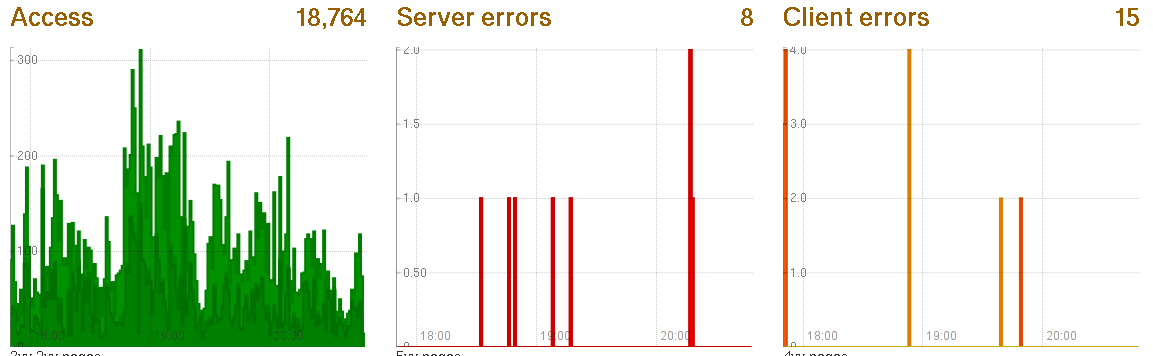
\includegraphics[width=11cm]{files/giraffe.png}\\
    \large
    Alternative to gdash
    \end{center}

}
\frame{%
\frametitle{Collectd}
    \begin{LARGE}
    \begin{itemize}
        \xitem{Statistics collection daemon}
        \xitem{{\color{inuits}A lot} of plugins available\ldots}
        \xitem{Can send data to graphite}
        \xitem{Simple configuration}
    \end{itemize}
    \end{LARGE}
}
\frame{%
\frametitle{Collectd plugins}
    \flushright{\tiny{\color{darkgrey}http://www.flickr.com/photos/juhansonin/3141561416/}}
    \begin{center}
        \includegraphics[height=4cm]{files/flickr_plugins.jpg}
    \end{center}
}
\frame{%
\frametitle{Collectd plugins}
\begin{small}
\begin{center}
\shadowtext{AMQP Apache APC\_UPS Apple\_Sensors Ascent Battery BIND Carbon}\\
\shadowtext{ConnTrack ContextSwitch CPU CPUFreq CSV cURL cURL-JSON cURL-XML}\\
\shadowtext{DBI DF Disk DNS E-Mail Entropy Exec FileCount FSCache GenericJMX}\\
\shadowtext{gmond HDDTemp Interface IPMI IPTables IPVS IRQ Java libvirt Load}\\
\shadowtext{LogFile LPAR MadWifi MBMon memcachec memcached Memory Modbus}\\
\shadowtext{Monitorus Multimeter MySQL NetApp Netlink Network NFS nginx}\\
\shadowtext{Notify\_Desktop Notify\_Email NTPd NUT olsrd OneWire OpenVPN OpenVZ}\\
\shadowtext{Oracle Perl Pinba Ping PostgreSQL PowerDNS Processes Protocols Python}\\
\shadowtext{Redis RouterOS RRDCacheD RRDtool Sensors Serial SNMP Swap SysLog}\\
\shadowtext{Table Tail Tape TCPConns TeamSpeak2 TED thermal TokyoTyrant UnixSock}\\
\shadowtext{Uptime Users UUID Varnish vmem VServer Wireless XMMS}\\
\shadowtext{Write\_Graphite Write\_HTTP Write\_MongoDB}\\
\shadowtext{Write\_Redis Write\_Riemann ZFS\_ARC}
\end{center}
\end{small}
}
\frame{%
\frametitle{Logstash}
    \begin{LARGE}
    \begin{itemize}
        \xitem{Ship logs from any source}
        \xitem{Filter them}
        \xitem{Index them}
        \xitem{Search them}
        \xitem{Backed with elasticsearch}
    \end{itemize}
    \end{LARGE}

}
\frame{%
\frametitle{Logstash}
    \begin{center}
        \includegraphics[height=7.5cm]{files/logstash.png}\\
    \end{center}
}
\frame{%
\frametitle{Kibana}
\begin{itemize}
\xitem{Kibana is a web interface for Logstash/ES}
\xitem{Kibana 1 was written in PHP}
\xitem{Kibana 2 was written in Ruby}
\xitem{Kibana 3 is written in AngularJS}
\end{itemize}
}
\frame{%
\frametitle{Kibana 3}
\begin{itemize}
\xitem{Everything happens in the browser}
\xitem{The browser is connected to Elasticsearch}
\xitem{You can save dashboards into ES}
\xitem{You can write/template dashboards to files}
\end{itemize}
}
\begin{frame}[fragile]
\frametitle{Kibana queries}
\begin{block}{Example of a kibana query}
\large
\begin{verbatim}
@fields.syslog_program:"httpd" AND
@fields.http_host:"test.example.com" AND
@fields.response:"404"
\end{verbatim}
\end{block}
\begin{itemize}
\xitem Lucene query syntax
\xitem Simple and effective
\xitem Point \& click web interface
\end{itemize}
\end{frame}

\frame{%
    \begin{center}
        \includegraphics[height=7.5cm]{files/kibana3.png}\\
    \end{center}
}
\frame{%
    \begin{center}
        \includegraphics[height=7.5cm]{files/kibana3b.png}\\
    \end{center}
}
\frame{%
\frametitle{Statsd}
    \begin{LARGE}
    \begin{itemize}
        \xitem{Graphite friend}
        \xitem{Stats aggregation}
        \xitem{Simple counters}
        \xitem{Flushes every XX seconds to graphite}
        \xitem{UDP}
    \end{itemize}
    \end{LARGE}
}
\begin{frame}[fragile]
\frametitle{Feeding statsd}
        \LARGE
\begin{verbatim}
echo "stats.sshd.login:1|c" |
nc -u statsd.example.com 8125
\end{verbatim}
\end{frame}
\frame{%
\frametitle{Toolchain example}
    \begin{large}
    \begin{itemize}
        \xitem{Apache ships logs to rsyslog}
        \xitem{Rsyslog ships logs to logstash}
        \xitem{Logstash ships metrics to statsd}
        \xitem{Statsd ships metrics to Graphite}
        \xitem{Icinga query metric from graphite}
        \xitem{https://github.com/etsy/nagios\_tools}
    \end{itemize}
    \end{large}
}
\frame{%
\frametitle{Reusing Icinga/Nagios perfdata}
    \begin{large}
    \begin{itemize}
        \xitem{Icinga performs various checks}
        \xitem{Icinga sends perfdata to graphite}
        \xitem{Graphite stores the data}
        \xitem{Gdash serves them inside dashboards}
        \xitem{https://github.com/roidelapluie/icinga-to-graphite}
    \end{itemize}
    \end{large}
}
\frame{%
\frametitle{Sharing}
\large
\begin{itemize}
\xitem{Build dashboard: dashing, teamdash}
\xitem{Share with developers}
\xitem{Share with managers}
\end{itemize}
}
\frame{%
\frametitle{Try them yourself}
\center{%
    \begin{large}
    \shadowtext{https://github.com/KrisBuytaert/vagrant-graphite}\\
    \end{large}
}
}
\begin{frame}
\frametitle{Thank you}
\begin{center}
\LARGE
\shadowtext{Any question?}
\end{center}
\end{frame}
\frame{%
\frametitle{Contact}
    \begin{columns}[T]
        \begin{column}{.5\textwidth}
    \begin{large}
    \shadowtext{Julien Pivotto}\\
    \shadowtext{julien@inuits.eu}\\
    \shadowtext{@roidelapluie}
    \end{large}
        \end{column}
        \begin{column}{.5\textwidth}
    \vspace{2cm}
    \begin{small}
    \includegraphics[height=2cm]{files/inuitslogo.png}\\
    \shadowtext{INUITS bvba}\\
    \shadowtext{Duboisstraat 50}\\
    \shadowtext{2060 Antwerp}\\
    \shadowtext{Belgium}\\
    \shadowtext{+32 473 441 636}\\
    \shadowtext{https://inuits.eu}
    \end{small}
        \end{column}
        \end{columns}
}
%{%
%\usebackgroundtemplate{}
%\setbeamercolor{background canvas}{bg=}
%
\includepdf{slides.pdf}
%}



%\begin{frame}
%\frametitle{}
%\begin{itemize}
%\xitem{}
%\end{itemize}
%\end{frame}
%\begin{frame}
%\frametitle{}
%\begin{itemize}
%\xitem{}
%\end{itemize}
%\end{frame}
%\begin{frame}
%\frametitle{}
%\begin{itemize}
%\xitem{}
%\end{itemize}
%\end{frame}
%\begin{frame}
%\frametitle{}
%\begin{itemize}
%\xitem{}
%\end{itemize}
%\end{frame}

\end{document}
